
% NC: Might need to have a think about how many tables and figures to include. Fine for thesis but please check JEB guidelines.
	%SF: Manuscript limit is 10 printed pages including figures and tables

	% NC: OK, so no limit to number of tables or figures?
	 % NC: Also see if they want Table and Figure or table and figure, or fig.	

%Start: 22/04/14
%Last edited on 19/08
	%01/08 Removed the simulations completely and changed the focus to more of a morphological study


% Preamble
% NC: I've reordered this a bit (but check it) so that stuff you'll always want is near the top
% and stuff you may need to change depending on the journal is near the bottom

\documentclass[12pt,a4paper]{article}
\usepackage{enumerate} 	% put in numbers or bullet points
\usepackage{setspace}	% line spacing					
\usepackage{authblk}	% For author affiliations
\usepackage{graphicx} 	% For adding pictures

\usepackage[nomarkers]{endfloat} %Figures and tables at the end of the document
\usepackage{pdflscape}	% for landscape pages
\usepackage{mathtools}	% For equations etc.
\usepackage[osf]{mathpazo} % palatino font package

\usepackage{ms}     	% load the manuscript style template

%\usepackage{float}		% Use these options to have figures in specific places in the text
%\floatstyle{plaintop} 	% Force table captions to go above the table

\setcounter{secnumdepth}{0} % removes numbers from section headings
\raggedright 			% justify the text on the left only
\pagenumbering{arabic}	% Page numbers

%\onehalfspacing 		%1.5 line spacing - use the below instead in case you need double spacing for some journals
%\linespread{1.6} 		% this is 1.5 spacing, double line spacing is 1.6 - unrecognised command (maybe due to the setspace package?)
\usepackage[round]{natbib} % author-year citations in round brackets

\title{Quantifying cranial morphological disparity in tenrecs (Afrosoricida, 	Tenrecidae) with implications for their designation as an adaptive radiation} 
% I want to come up with a better title

\author{Sive Finlay$^{1,2,*}$ and Natalie Cooper$^{1,2}$}
\affiliation{\noindent{\footnotesize
$^1$ School of Natural Sciences, Trinity College Dublin, Dublin 2, Ireland.\\ 
$^2$ Trinity Centre for Biodiversity Research, Trinity College Dublin, Dublin 2, Ireland.\\
$^*$Corresponding author: sfinlay@tcd.ie; Zoology Building, Trinity College Dublin, Dublin 2, Ireland.\\ Fax: +353 1 6778094; Tel: +353 1 896 2571.\\}}
\date{}	% To give blank date

\runninghead{Cranial morphological disparity in tenrecs} %I'll fix this when I have a proper title

\keywords{disparity, morphology, geometric morphometrics, tenrecs, golden moles, adaptive radiation}

% Start of document
\begin{document}

\modulolinenumbers[1] 	% Line numbering on every line

\mstitlepage			% Instead of \maketitle you can use the nice template to get it looking like a manuscript
\parindent=1.5em		% Changes paragraph indenting so it's not so big
\addtolength{\parskip}{.3em} % Changes spacing between sections so it's smaller
%---------------------------------------------------
\begin{abstract} %NC: Mostly I've made this more concise. Try not to over write things, keep it simple. 

	Understanding why some clades are more phenotypically diverse than others remains a central challenge in evolutionary biology. This issue is particularly relevant when we consider whether a group represents an adaptive radiation. However, we must be able to identify exceptionally diverse clades before we can determine the selective pressures which led to the evolution of their variety. Tenrecs (Afrosoricida, Tenrecidae) are a family of small mammals and are often cited as an example of a phenotypically diverse, adaptively radiated group. However, this assumption has not been tested. Here we use geometric morphometric analyses of cranial and mandible shape to test whether tenrecs show exceptional morphological disparity. We find that tenrecs are no more morphologically diverse than their sister taxa, the golden moles (Afrosoricida, Chrysochloridae), casting doubt over whether tenrecs should be considered to be an exceptionally diverse group. 
%NC: I don't like the last sentence. It's basically just a repeat of the previous sentence.
	%Our results reveal new insight into patterns of morphological variety within tenrecs and the question of whether apparent phenotypic diversity is more than skin deep.
%SF: So maybe I don't need a final alternative?


\end{abstract}

\newpage
%-------------------------------------------------------
\section{Introduction} 
%SF: I took out the vague paragraph about studies that quantify phenotypic variety -> straight into adaptive radiations instead.
	Phenotypically diverse groups have long attracted the attention of evolutionary biologists, particularly when it comes to the study of adaptive radiations - `evolutionary divergence of members of a single phylogenetic lineage into a variety of different adaptive forms' \citep[Futuyma 1998, cited by][]{Losos2010}. 

	There are many famous examples of adaptive radiations including Darwin's finches, Caribbean \textit{Anolis} lizards and cichlid fish \citep{Gavrilets2009}. However, there has been considerable debate about how adaptive radiations should be defined \citep{Glor2010, Losos2010a} based on the relative importance of speciation rates, species richness and morphological diversity. One particular issue is whether it is even meaningful to distinguish a specific group of species as an adaptive radiation or not based on arbitrary statistical thresholds of variety \citep{Olson2009}.
	%SF: Re-phrased the laste sentence to try and make it clearer

	Despite the controversies and disagreements, there does seem to be a consensus that high morphological diversity is an important criterion for identifying adaptive radiations \citep{Losos2010a, Olson2009}. One way to test whether a group shows high morphological diversity is through sister taxa comparisons. For example, Losos and Miles (\citeyear{Losos2002}) used this approach to demonstrate exceptional diversity in some but not all clades of iguanid lizards. This is a good way of assessing the relative diversity of a clade but of course there is also a danger that a focal clade's diversity will be judged to be exceptional just because it is more variable than an exceptionally non-diverse sister taxon \citep{Losos2002}. 

%Still needs another linking sentence here
%COME BACK TO HERE

	Here we use sister-taxa comparisons to test whether tenrecs (Afrosoricida, Tenrecidae) exhibit the high levels of phenotypic diversity that are expected of an adaptively radiated clade.
	% NC: Yeah this paragraph needs some work. Jumps quite quickly from really broad to really focused. 

% SF: Shorter tenrec paragraph

	The tenrec family contains 34 species, 31 of which are endemic to Madagascar \citep{Olson2013}. Tenrecs are often cited as an example of an adaptively radiated family which exhibits exceptional morphological diversity \citep{Soarimalala2011, Olson2003}. Body sizes of extant tenrecs span three orders of magnitude (2.5 to $>$ 2,000g) which is a greater range than all other Families, and most Orders, of living mammals \citep{Olson2003}.
		% NC Could alternatively cite the PanTHERIA dataset here 	
			%SF: Yep, I just put this reference in because that's where I got the claim that the range is greater than any other Family but I guess it's easy enough to check in PanTHERIA too
	Within this vast size range there are tenrecs which convergently resemble shrews (\textit{Microgale} tenrecs), moles (\textit{Oryzorictes} tenrecs) and hedgehogs (\textit{Echinops} and \textit{Setifer} tenrecs) \citep{Eisenberg1969} even though they are not closely related to these species \citep{Stanhope1998}.

	However, evidence for claim that tenrecs are exceptionally diverse has not been tested. Here we present the first quantitative investigation of morphological diversity in tenrecs, and how this compares to their closest relatives, the golden moles (Afrosoricida, Chryscholoridae). 
	We apply two dimensional geometric morphometric techniques \citep{Rohlf1993, Adams2013} to create morphospace plots that depict cranial and mandible morphological variation in the two Families. We use these morphospaces to compare the relative morphological disparity \citep{Foote1997, Wills1994, Erwin2007} within each Family. 
	
% NC: I find the idea of defining disparity like this a bit odd. When I say define disparity I mean HOW are you measuring disparity? If you're looking at differences isn't it always going to be disparity? 
% NC: Again I think this paragraph can be combined with the one before. Doesn't really matter that there are different ways to measure disparity, and you can get away with just defining in the methods I think.

%SF: I took out the different disparity methods and combined the other information with the previous paragraph

	%Disparity can be calculated in many ways including measures of morphospace occupation \citep[e.g.][]{Goswami2011, Brusatte2008} and rate-based approaches that assess the amount of directed change away from an ancestor \citep{OMeara2006, Price2013}. Here we focus on patterns of phenotypic variety in extant species rather than analysing the rate of diversity accumulation through time. 


	Our results show an overall trend for higher morphological diversity in tenrec crania compared to those of golden moles. However, these differences are not statistically significant. These findings indicate that, with regards to cranial shape, tenrecs are no more morphologically diverse than their closest relatives. 
	
	% SF: Changed it so I'm only making claims about tenrec diversity compared to golden moles rather than lots of groups.
	
	In contrast, we found significantly greater morphological disparity in golden mole mandibles compared to tenrecs. 
	%seemingly due to more variable posterior mandible morphologies in golden moles. 
	% NC: This is a bit technical for the intro
	% SF: Grand, I kept in the claim but removed the technical reason, or should I just take the whole mandibles part out?
	These findings cast doubt over whether the apparent phenotypic diversity within tenrecs should be considered to be truly exceptional. 


%-------------------------------------------------------------
\section{Materials and Methods}

\subsection{Morphological data collection} 

	%I've changed to including all 4 views in the main text of the paper because I had some more room after taking out the simulations. I think it makes more sense to have all of them together instead of separated in the paper and supplementary.
	
	One of us (SF) photographed cranial specimens of tenrecs and golden moles at the Natural History Museum London (BMNH), the Smithsonian Institute Natural History Museum (SI), the American Museum of Natural History (AMNH), Harvard's Museum of Comparative Zoology (MCZ) and the Field Museum of Natural History, Chicago (FMNH). We photographed the specimens with a Canon EOS 650D camera fitted with an EF 100mm f/2.8 Macro USM lens using a standardised procedure to minimise potential error (see supplementary material for details). 
	%NC Might want to use the standard museum abbreviations - BMNH etc.
		%SF I used NHML because I thought the BMNH was the old name?
		% NC: Nope, it's the standard museum name for specimens. Doesn't really matter.
		%SF: Grand, I changed it in the text but my pictures are labelled NHML so I can just put a note with the figshare folder

	We collected pictures of the skulls in dorsal, ventral and lateral views (right side of the skull) and of the outer (buccal) side of the right mandibles. A full list of museum accession numbers and details on how to access the images can be found in the supplementary material.
	%AMNH and SI pictures are on figshare but MCZ and FMNH are more tricky about copyright so I haven't put those pictures up
	% NC: May be worth linking to figshare here rather than just in suppl
	
	%COME BACK FOR THE FIGSHARE REFERENCE

	In total we collected pictures from 182 skulls in dorsal view (148 tenrecs and 34 golden moles), 173 skulls in ventral view (141 tenrecs and 32 golden moles), 171 skulls in lateral view (140 tenrecs and 31 golden moles) and 182 mandibles in lateral view (147 tenrecs and 35 golden moles), representing 31 species of tenrec (out of the total 34 in the family) and 12 species of golden moles (out of a total of 21 in the family \citep{Asher2010}). We used the taxonomy of Wilson and Reeder \citeyearpar{Wilson2005} supplemented with more recent sources \citep{IUCN2012, Olson2013} to identify our specimens. 
	

	We used a combination of both landmarks (type 2 and type 3, \citep{Zelditch2012}) and semilandmarks to characterise the shapes of our specimens. Figure \ref{fig:skdors_skvent_landmarks} shows our landmarks (points) and semilandmarks (outline curves) for the skulls in dorsal and ventral views and figure \ref{fig:sklat_mands_landmarks} shows the points and curves we used for lateral views of skulls and mandibles. Corresponding definitions of each of the landmarks can be found in the supplementary material.
	
	%semilandmark or semi-landmark? The Latter might improve readability
	%SF: it's usually semilandmark in other papers

	We digitised all landmarks and semilandmarks in tpsDIG, version 2.17 \citep{Rohlf2013}. We re-sampled the outlines to the minimum number of evenly spaced semilandmark points required to represent each outline accurately \citep[][details in supplementary material]{MacLeod2013}. We used TPSUtil \citep{Rohlf2012} to create sliders files \citep{Zelditch2012} to define which points were semilandmarks. We conducted all subsequent analyses in R version 3.0.2 \citep{Team2014} within the geomorph package \citep{Adams2013}. We used the gpagen function to run a general Procrustes alignment \citep{Rohlf1993} of the landmark coordinates while sliding the semilandmarks by minimising Procrustes distance \citep{Bookstein1997}. We used these Procrustes-aligned coordinates of all species to calculate average shape values for each species (n = 43) which we then used for a principal components (PC) analysis with the plotTangentSpace function \citep{Adams2013}. 

%*************************************************
%May need to re-do pictures to grey scale instead of colour
% NC: Yep you'll need those for the publication I think
%**************************************
%Skdors and skvent
	%landmarks diagram
	\begin{figure}
	\centering
	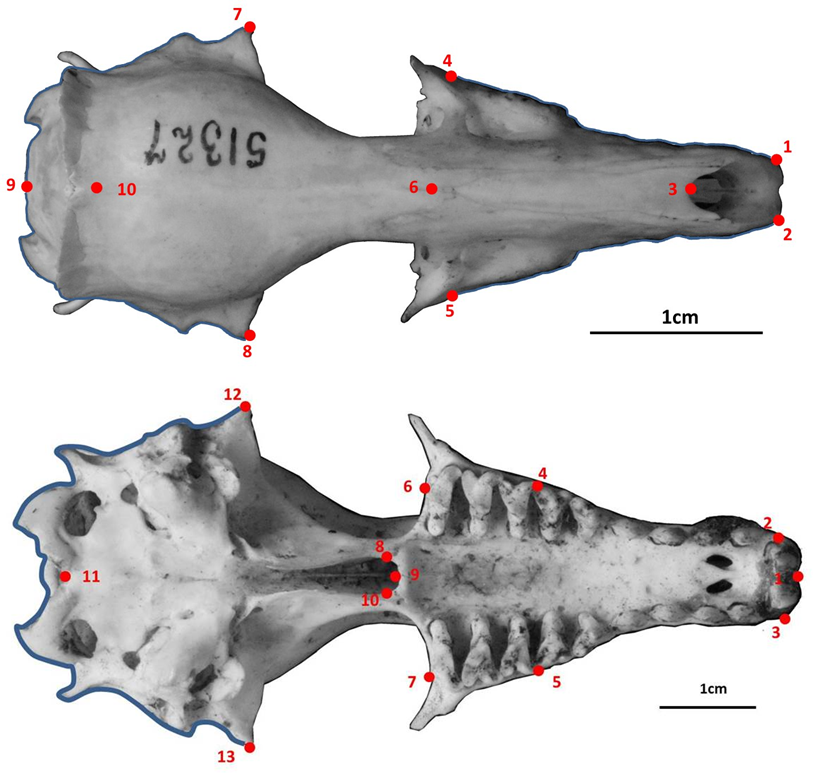
\includegraphics[width=1\linewidth]{figures/SkDors+Skvent_landmark_diagrams.png}
	
	\caption[Diagram of the landmarks and curves for the skulls in dorsal and ventral views]
		{Landmarks (red points) and curves (blue lines) used to capture the morphological shape of skulls in dorsal and ventral views respectively. Curves were re-sampled to the same number of evenly-spaced points. See Supplementary Material for descriptions of the curves and landmarks. The specimens belong to two different \textit{Potamogale velox} (Tenrecidae) skulls: accession number AMNH 51327 (dorsal) and NHML 1934.6.16.2 (ventral)}
	
	\label{fig:skdors_skvent_landmarks}
	\end{figure}


%Mandibles and Skulls lateral
	%landmarks diagram
	\begin{figure}[H]
	\centering
	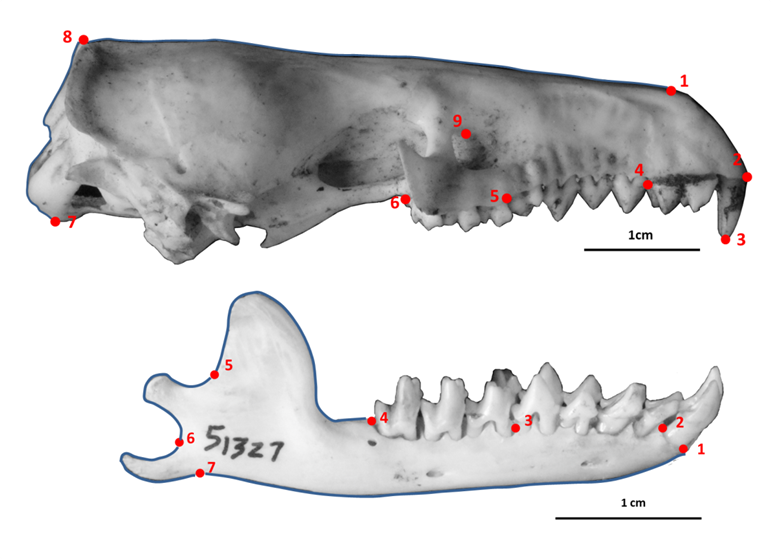
\includegraphics[width=1\linewidth]{figures/SkLat+mands_landmark_diagrams.png}
	
	\caption[Diagrams of the landmarks and curves used for lateral views of skulls and mandibles]
		{Landmarks (red points) and curves (blue lines) used to capture the morphological shape of lateral views of skulls and mandibles respectively. Curves were re-sampled to the same number of evenly-spaced points. See Supplementary Material for descriptions of the curves and landmarks. The specimens belong to two different \textit{Potamogale velox} (Tenrecidae) skulls: accession number AMNH 51327 (dorsal) and NHML 1934.6.16.2 (ventral)}
	
	\label{fig:sklat_mands_landmarks}
	\end{figure}
%

%************************************************** 
%I'm no longer using the phylogenies for comparing disparity in the two families - they were just for the simulations part

%I don't know if it's necessary to do phylogenetic PCAs since I'm already basing all of my comparisons on family divisions?

% NC: Probably technically you should do phylogenetic PCAs. Read Liam's paper on them. But also Matt's one I sent you the other week. For now though just do normal PCAs. The point is not how you separate species, the point is that the PCA scores will be biased by where the species sit in the phylogeny.

	%COME BACK TO HERE AND TRY PHYLOGENETIC PCAs

%\subsubsection{Phylogeny} 
	%Instead of basing our analyses on individual trees and assuming that their topologies were known without error \citep[e.g.][]{Ruta2013, Foth2012, Brusatte2008, Harmon2003} we used a distribution of 101 pruned phylogenies derived from the randomly resolved mammalian supertrees in \citep{Kuhn2011}. 
		% I used 101 because that was the number in the smaller Fritz file - I could change it to 100 instead if 101 sounds odd?

	%Eight species (six \textit{Microgale} tenrecs and two golden moles) in our morphological data were not in the phylogenies. Phylogenetic relationships among the \textit{Microgale} have not been resolved more recently than the \citep{Kuhn2011} analysis, therefore we added the additional \textit{Microgale} species at random to the \textit{Microgale} genus within each phylogeny \citep{Revell2012}. We could not use the same approach to add the two missing golden mole species because they were the only representatives of their respective genera within our data. Therefore we randomly added these species to the common ancestral node (using the findMRCA function in phytools \citep{Revell2012}) of all golden moles within each phylogeny. Adding these extra species to the phylogenies created polytomies which we resolved arbitrarily using zero-length branches \citep{Paradis2004}. We calculated pairwise phylogenetic distances among species using the cophenetic function \citep{Team2014}. 
	% NC: I feel like some of this belongs in the analysis section...
		%SF Me too but I'm not sure where to put it without making a separate analyses section for the phylogenies and I don't think that makes sense.  
	
%-------------------------------------------------------	
\subsection{Disparity calculations}
%Come back to re-write this section to try and make it clearer

	We calculated morphological disparity separately for golden moles and tenrecs in each of the morphological datasets. We used the PC axes which accounted for 95\% of the cumulative variation to calculate four disparity metrics; 1) the sum of the range, 2) the product of the range, 3) the sum of the variance and 4) the product of the variance of morphospace occupied by each Family \citep{Brusatte2008, Foth2012, Ruta2013}. 

	%We also calculated morphological disparity directly from the Procrustes-superimposed shape data based on the sum of the squared inter-landmark distances between the average shape of a species and the overall grand mean shape \citep[SSqDist,][]{Zelditch2012}. 
% NC: Need to explain more carefully. This read like you copied it directly from a paper i.e. that you don't understand what you've done.
%SF: I'm just removing this metric completely because it only makes both me and the paper more confused

	We used two approaches to test whether tenrecs have significantly different morphologies compared to golden moles. First we compared morphospace occupation between the two groups with non parametric MANOVAs \citep{Anderson2001} to test whether tenrecs and golden moles occupy significantly different areas of morphospace \citep[e.g][]{Serb2011, Ruta2013}.
	 
	Secondly, we tested whether tenrecs have significantly higher or lower disparity than golden moles. If the two Families have equal disparity then the designation of each species as being either a tenrec or golden mole should not make any difference to our calculations. Therefore we used pairwise permutation tests to assess whether our data differed from this null hypothesis. We assigned Family identities at random to each specimen and calculated the differences in disparity for these new Family groupings. We repeated these permutations 1000 times to generate a null distribution of the expected differences in Family disparity. We compared our observed (true) measures of the differences in disparity between tenrecs and golden moles to these permuted distributions to test whether the families had significantly different levels of disparity compared to the null hypothesis.

% SF: I tried re-writing this disparity methods explanation, not sure if it makes it any clearer though

	The majority of tenrec species (19 out of 31 in our dataset) are members of the \textit{Microgale} (shrew-like) Genus which is notable for its relatively low phenotypic diversity \citep{Soarimalala2011, Jenkins2003}. The strong similarities among these species may mask signals of higher disparity among other tenrecs. Therefore we repeated our Family-level comparisons of disparity excluding the \textit{Microgale} species so that we could compare disparity within the remaining 12 tenrec species to disparity within the 12 species of golden moles.

% NC: Now this is shortened I'd stick the rarefaction in here too
	% SF: I took out rarefaction because Steve Wang and Steve Brusatte both advised that it was not the most appropriate test to use. The permutation method also takes sample size into account so I thought that removed the need for a rarefcation analysis aswell?
%-----------------------------------------------------------

\section{Results}


\subsection{Morphological disparity in tenrecs and golden moles} 
 
	Figure  \ref{fig:fourPCA} depicts the morphospace plots derived from our principal components analyses of average Procrustes-superimposed shape coordinates for each species in our skull and mandible data respectively. We used the principal components axes which accounted for 95\% of the cumulative variation (number of axes: n = 7 (dorsal), n = 8 (ventral), n = 8 (lateral) and n = 12 (mandibles)) to calculate the disparity of each Family. 

	Tenrecs and golden moles clearly have very different cranial and mandible morphologies: in each analysis, the families occupy significantly different areas of morphospace (npMANOVA, table \ref{tab:npmanova.summary}). Our comparisons of disparity within each Family yielded different trends for skulls compared to mandibles. In our analyses of the three different views of the skulls, there is an overall trend for tenrecs to have higher disparity than golden moles. However, none of these differences are statistically significant (table \ref{tab:disp.summary}). 
	
	%SF: I removed the SSqDist method because it was just causing confusion
	%In contrast, when we calculated disparity based on the squared inter-landmark distances between the average shape of a species and the overall grand mean shape \citep{Zelditch2012} then golden moles had significantly higher disparity than tenrecs (table \ref{tab:disp.summary}). These results indicate that golden moles are more distant from the overall mean shape in each of the analyses (farther from the (0,0) points in the PCA plots, see figure \ref{fig:fourPCA}) which makes intuitive sense given that the overall mean shape in each analysis will necessarily be biased towards the more species-rich tenrec Family. 
	
	%I'm not sure if this is the right interpretation of the SSqDist results because I thought the permutation tests take sample size differences into account? 
	%I could just take out this extra metric completely to avoid confusion

	% NC: Up to you. I don't like the way you explain it in the methods either so it might be easier to remove it at this point.
	
	
	There is a less clear pattern from our analysis of disparity in mandibles. Three of our four metrics indicate that golden moles have significantly higher disparity in the shape of their mandibles than tenrecs (table \ref{tab:disp.summary}) although one metric (sum of ranges) indicated the opposite result. 
	
	The three curves at the back of the mandibles (figure \ref{fig:sklat_mands_landmarks}) place a particular emphasis on shape variation in the posterior of the bone; the ramus, coronoid, condylar and angular processes. Therefore, higher disparity in golden mole mandibles compared to tenrecs could be driven by greater morphological variation in these structures. To test this idea, we repeated our morphometric analyses of the mandibles with a reduced dataset of points; just the seven landmark points and one single curve at the base of the jaw between landmarks 1 and 7 (figure \ref{fig:sklat_mands_landmarks}). When we compared disparity with this reduced data set we found that golden moles no longer had significantly higher disparity than tenrecs (table \ref{tab:disp.summary}).
	
\subsection{Morphological disparity in non-\textit{Microgale} tenrecs and golden moles} 	   
	We repeated our disparity comparisons with a subset of the tenrec specimens to remove the large and phenotypically similar \textit{Microgale} tenrec Genus. In this case we found that tenrecs have significantly higher disparity than golden moles when the skulls are analysed in lateral view (table \ref{tab:disp.nonmic.summary}). However, none of the other comparisons in any of the analyses were significant. 


%************************************
%Results tables and figures

%Summary table of the Family comparisons for all tenrecs vs. golden moles
	\begin{table}[h]			
	\caption[Summary of disparity comparisons between tenrecs and golden moles]
		{Disparity comparisons between tenrecs (T) and golden moles (G) for each of our data sets(rows) and four disparity metrics (columns). `Mandibles:one curve' refers to our shape analysis of mandibles excluding the three curves around the posterior structures of the jaw (figure \ref{fig:sklat_mands_landmarks}). Significant differences are highlighted in bold with the corresponding p value in brackets. Disparity metrics are: sum of variance, product of variance, sum of ranges and product of ranges }
	\centering
	%Disparity family comparison results summary
%All tenrecs and golden moles

\begin{tabular}[t]{l l l l l l }		
\hline
\textbf{Disparity metric} & \textbf{SumVar} & \textbf{ProdVar} & \textbf{SumRange} & \textbf{ProdRange} & \textbf{SSqDist} \\
\hline
Skulls dorsal & T$>$G & T$>$G & T$>$G & T$>$G &	\textbf{G$>$T* (0)}\\
%-----------------------------------------------------------
Skulls lateral	& T$>$G & T$>$G & T$>$G & T$>$G & \textbf{G$>$T* (0)}\\
%-------------------------------------------------------
Skulls ventral & T$>$G & G$>$T & T$>$G & T$>$G & \textbf{G$>$T* (0)}\\
%-------------------------------------------------------
Mandibles & G$>$T & \textbf{G$>$T* (0.008)} & \textbf{T$>$G* (0.025)} & \textbf{T$>$G* (0.009)} &	\textbf{T$>$G* (0)}\\
%-------------------------------------------------------
Mandibles: one curve & G$>$T & G$>$T & T$>$G & T$>$G &	\textbf{T$>$G* (0)}\\
%-------------------------------------------------------
\hline
\end{tabular} 
	\label{tab:disp.summary}  
	\end{table}

%Summary of the Family comparisons for non-Microgale tenrecs vs. golden moles
	\begin{table}[h]			
	\caption[Summary of disparity comparisons between non-\textit{Microgale} tenrecs and golden moles]
		{Disparity comparisons between non-\textit{Microgale} tenrecs (T) and golden moles (G) for each of our data sets(rows) and four disparity metrics (columns). Significant differences are highlighted in bold with the corresponding p value in brackets. Disparity metrics are; sum of variance, product of variance, sum of ranges and product of ranges. }
	\centering
	%Disparity family comparison results summary
%Non-Microgale tenrecs and golden moles

\begin{tabular}[t]{l l l l l l }		
\hline
\textbf{Disparity metric} & \textbf{SumVar} & \textbf{ProdVar} & \textbf{SumRange} & \textbf{ProdRange} & \textbf{SSqDist} \\
\hline
Skulls dorsal & T$>$G & T$>$G & T$>$G & T$>$G &	T$>$G\\
%-----------------------------------------------------------
Skulls lateral	& T$>$G* (0.014) & T$>$G & \textbf{T$>$G* (0.001)} & \textbf{T$>$G*(0.003)} & \textbf{G$>$T* (0.014)}\\
%-------------------------------------------------------
Skulls ventral & T$>$G & T$>$G & T$>$G & T$>$G & T$>$G\\
%-------------------------------------------------------
Mandibles & T$>$G & G$>$T & T$>$G & G$>$T &	G$>$T\\
%-------------------------------------------------------
%Don't need to do a subset analysis of mandibles for non-Microgale tenrecs
%Mandibles one curve & G$>$T & T$>$G & T$>$G & T$>$G & G$>$T\\
%-------------------------------------------------------
\hline
\end{tabular} 
	\label{tab:disp.nonmic.summary}  
	\end{table}
	
%Summary table of the npMANOVA morphospace occupation comparisons
	
	\begin{table}[h]			

	\caption[Summary of npMANOVA comparisons of morphospace occupation for tenrecs and golden moles]
		{npMANOVA comparisons of morphospace occupation for tenrecs and golden moles in each of the four analyses (three views of skulls and mandibles). In each case the two families occupy significantly different areas of morphospace.}
	\centering
	
%All tenrecs and golden moles
%npMANOVA results summary
%Values from the _manova.res files: npMANOVA based on the PC axes (not distance matrices)

\begin{tabular}[t]{l l l l }		
\hline
\textbf{Analysis} & \textbf{F} & R$^2$ & p value \\
\hline
Skulls dorsal & 66.02 & 0.62 & 0.001 \\
%-------------------------------------------
Skulls ventral & 100.74 & 0.71 &0.001 \\
%------------------------------------------
Skulls lateral & 75.07 & 0.65 & 0.001 \\
%------------------------------------
Mandibles & 59.34 & 0.59 & 0.001 \\
%-------------------------------------------------------
\hline
\end{tabular} 
	\label{tab:npmanova.summary}  
	\end{table}
		
%PCA figures: changed to having all four plots instead of individual PCA graphs
	%Source of this figure in my shape_data/output folder 
	\begin{figure}[H]
	\centering
	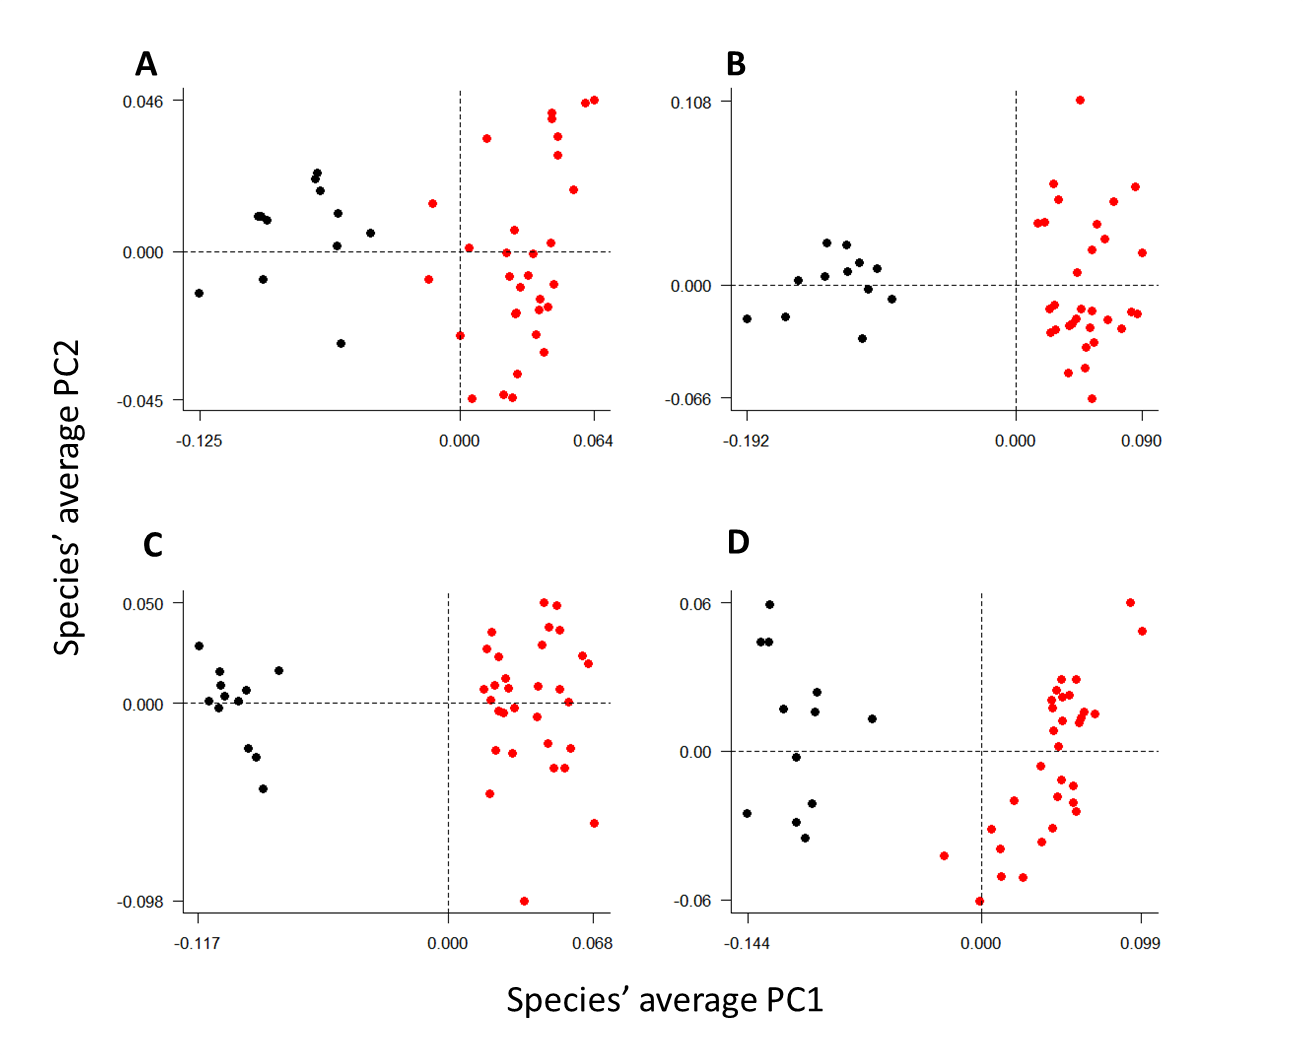
\includegraphics[width=1\linewidth]{figures/FourPlotPCA.png}
	\caption[Principal components plots of the morphospaces occupied by tenrecs and golden moles]
		{Principal components plots of the morphospaces occupied by tenrecs (red, n = 31 species) and golden moles (black, n = 12) for the skulls: dorsal (A), ventral (B), lateral (C) and mandibles (D) analyses. Axes are PC1 and PC2 of the average scores from a PCA analysis of mean Procrustes shape coordinates for each species. }
	\label{fig:fourPCA}
	\end{figure}
%**********************************************


\section{Discussion} 

% NC: OK this section needs another proper go over. I don't get what you're trying to say in most places. Worth going back to the intro and making sure you draw in all the themes you touch on there. So your concluding remarks should be about adaptive radiation. Try writing this discussion again, using the same techniques as for writing introductions. Except the direction is narrow to broad rather than broad to narrow. Have a reason for each paragraph, a story you want to tell.

%1) Specific discussion of results and differences between skulls and mandibles
	Our analyses are the first quantitative investigation of morphological disparity in tenrecs. We show that tenrecs' cranial morphologies are no more diverse than their closest relatives and therefore phenotypic variety in tenrecs is perhaps not as exceptional as it first appears.
	
	One apparent anomaly in our results is that we found opposite patterns of disparity among tenrecs and golden moles in the analyses of skulls and mandibles.
	
	When we compared the diversity of skull shapes in the two Families, we found a trend towards higher disparity in tenrecs compared to golden moles but none of these differences were significant (table \ref{tab:disp.summary}). Even when we removed the phenotypically similar \textit{Microgale} Genus, tenrecs were still no more diverse than golden moles in most of the analyses of their skull shapes (table \ref{tab:disp.nonmic.summary}). 
	
	In contrast to these patterns from the skull analyses, two of our disparity metrics indicate that golden moles have more disparate mandible shapes than tenrecs (table \ref{tab:disp.summary}).
	We recognised that our landmarks and curves for the mandibles focus particular attention on the ascending ramus (condyloid, condylar and angular processes, figure \ref{fig:sklat_mands_landmarks}). Therefore we deleted the three semilandmark curves around these structures and repeated our disparity calculations. In this case we found no significant difference in disparity between the two Families (table \ref{tab:disp.summary}). Therefore, our results seem to indicate that golden moles have greater morphological variation in the posterior structures of their mandibles compared to tenrecs.
		
	%I asked for advice from Gary Bronner about why I was getting higher variation in golden mole mandibles compared to tenrecs. He thinks that the most likely reason is a problem with my landmarks. Landmark 4 is the alveolus of the last molar but that position is not homologous across species because of the presence/absence of a third molar. His advice was to re-run the analysis without landmark 4 and curve A and see what patterns of shape variation come out then.
		
	%However, as I was choosing the landmarks I knew that the dental formulae varied for each species - and therefore the landmarks are relative points showing the end of the tooth row rather than biologically meaningful positions of dental characteristics. But now I don't know if I can get away with using that as an excuse when it comes to trying to explain strange results in my paper.
			
	 Given that these posterior structures act as muscle attachment and articulation sites for connections with the upper jaw %needs a ref
	 one might expect that golden moles with highly disparate posterior mandible morphologies should also show high variability in the corresponding mandible articulation areas of the skull. However, we could not locate reliable, homologous points accurately on those areas of the skull pictures in lateral view. Instead, our landmarks and semilandmark curves for the skulls in lateral view focus attention on morphological variation in the dentition and the overall shape of the top and back of the skulls (figure \ref{fig:sklat_mands_landmarks}). This may explain why golden mole skulls in lateral view do not show the same pattern of higher disparity compared to tenrecs that we see in our analyses of the mandibles. However, further investigation is required to identify possible reasons why golden moles appear to show such variation in the posterior structure of their mandibles.
	 	%SF: I know this is a weak ending but I'm still figuring out possible reasons for this pattern that aren't just data problems. 
	 	
		%The discrepancies could arise from factors associated with the modularity of morphological evolution.
	
		%There is strong evidence that morphological variation in skulls and mandibles is derived from differential evolution of integrated developmental modules \citep[reviewed by][]{Klingenberg2013a}.
		%For example, there seems to be two primary modules in the mouse mandible; an alveolar part which holds the teeth and the ascending ramus for muscle attachment and which articulates with the skull \citep{Klingenberg2008a}. Geometric shape covariation is stronger within rather than between these modules. 
	
	% NC: I don't really get the relevance of this part...
	% SF: It was just one of my ideas for trying to figure out why I'm getting different patterns in the mandibles compared to the skulls but I didn't manage to develop it properly
	
%------------------------------------------------------	
%2) Skulls are only one way of looking at diversity but it's still interesting to see that ecologically diverse tenrecs are no more disparate than the functionally similar golden mole family
	
	We used variation in skull and mandible shapes as proxy measures for overall morphological diversity within the two Families. Many other studies also use skulls to study phenotypic variation within species \citep{Blagojevic2011, Bornholdt2008}, to delineate species boundaries within a clade \citep[e.g.][]{Panchetti2008} or for cross-taxonomic comparative studies of phenotypic (dis)similarities \citep[e.g.][]{Ruta2013, Goswami2011, Wroe2007}.
	
	However, studies of morphological disparity are inevitably constrained to measure diversity within specific traits rather than overall phenotypes \citep{Roy1997}. Disparity calculations based on skull shape can yield similar results compared to analyses of whole-skeleton discrete characters and limb proportion data sets \citep{Foth2012}. Yet it is still possible that comparing disparity in tenrecs and golden moles using non-cranial morphological measures could produce different results. For example, tenrecs inhabit a wide variety of ecological niches and habitats including terrestrial, arboreal, semi-aquatic and semi-fossorial environments \citep{Soarimalala2011}. In contrast, although golden moles occupy a wide altitudinal, climatic and vegetational spectrum of habitats \citep{Bronner1995}, they are are all fossorial species which, superficially at least, appear to be less functionally diverse than tenrecs. Therefore, comparing the disparity of limb morphologies within the two Families could indicate that tenrecs have more morphologically diverse limbs than golden moles. 
	
	
%------------------------------------------
%Wider relevance to adaptive radiation

 	Evidence of exceptional morphological diversity is one criterion for designating a clade as an adaptive radiation \citep{Losos2010a}. Our analyses are the first measures of morphological diversity within tenrecs, a group which is commonly cited as an example of an adaptive radiation \citep{Olson2013}. We found that tenrecs are no more morphologically diverse than their their closest relatives and therefore, within our tests, do not appear to be exceptionally diverse.   
 	
 	The evolution of cranial shape (both upper skull and mandible), particularly dental morphology, has obvious correlations with dietary specialisations and occupation of specific ecological niches \citep[e.g.][]{Wroe2007}. Considering the wide ecological diversity of the tenrec Family; semi-fossorial, arboreal, terrestrial and semi-aquatic \citep{Soarimalala2011}, we think that it is reasonable to expect that this variety should be reflected in skull morphology. However, we have not included any measures of the `adaptiveness' of cranial shape in our analyses and therefore our analyses should not be considered to be an explicit test of whether or not tenrecs are an adaptive radiation \citep{Losos2010a}. Instead we have made the first step towards understanding the apparent phenotypic diversity within tenrecs within a quantitative framework. Future work should focus on explicit measures of the `adaptiveness' and functional importance of tenrec cranial and post-cranial morphologies to understand the significance of morphological diversity within the Family \citep[e.g.][]{Mahler2010}. However, we also recognise that strict, statistically based categorisations of clades as being adaptive radiations or not is not necessarily biologically meaningful or helpful when it comes to trying to understand patterns of phenotypic diversity \citep{Olson2009}.   


%---------------------------------------------------	
%4) Conclusions
	We have presented the first quantitative study which tests the common claim that tenrecs are an exceptionally diverse group \citep{Olson2013, Soarimalala2011,Eisenberg1969}. Focusing on cranial diversity is only one aspect of morphological variation and further analyses are required to test whether other morphological traits yield similar patterns. However, our results provide a clear indication that phenotypic variety within tenrecs is perhaps not as exceptional as it first seems.   
	
\section{Acknowledgements}

	We thank Fran\c{c}ois Gould, Dean Adams, David Polly, Gary Bronner, Steve Brusatte, Steve Wang, Luke Harmon, Thomas Guillerme and the members of NERD club for insightful discussions and the museum 
	staff and curators for their support and access to collections. Funding was provided by an Irish Research Council EMBARK Initiative Postgraduate Scholarship (SF) and the European Commission CORDIS Seventh Framework Programme (FP7) Marie Curie CIG grant. Proposal number: 321696 (NC)

\bibliographystyle{jeb}
\bibliography{refs_disparity}
% I downloaded the jeb.bst file from http://schneider.ncifcrf.gov/latex.html but there isn't an associated style file

% NC: You can make one via the command line as I showed you in one of my LaTeX lessons.

	%**********************
	%SF: I still need to do this so that the references have the abbreviated journal titles, don't include the doi and so that book references don't have the total number of pages but do have the editors' names
	%*******************************************




\end{document}